%codigo de latex funcion con secciones, imagenes, tablas, ecuaciones
%las fotos png deben estar en la misma carpeta que el documento




\documentclass[12pt, a4paper]{article}

% --- BASIC PACKAGES ---
\usepackage[utf8]{inputenc}
\usepackage[english]{babel}
\usepackage{graphicx}   % To insert images
\usepackage{amsmath}    % For math formulas
\usepackage{tikz}
\usepackage{pgfplots}
\pgfplotsset{compat=1.18}



% --- DOCUMENT METADATA ---
\title{\textbf{Technical Report: Week 1}}
\author{Student C: Commercial Center Project}
\date{September 22, 2025}



% =================================================================
% --- DOCUMENT START ---
% =================================================================
\begin{document}

% Page 1: Title
\maketitle

% Page 2: Table of Contents
\newpage
\tableofcontents
\newpage

% --- MAIN CONTENT ---
\section{Introduction}

This report details the resolution of the problems corresponding to **Week 1** of the Block 2 project: "Electrical Lines and Distribution Networks". The objective assigned to Student C is the design of a mixed (overhead/underground) distribution network for a commercial center.

\section{Problem 1: Line Classification and Selection}

\subsection{Line Classification}
The lines were classified according to their voltage level, application, and topology, as summarized in Table \ref{tab:classification}.

\begin{table}[htbp]
    \centering
    \caption{Line Classification for the Commercial Center.}
    \label{tab:classification}
    \begin{tabular}{|l|l|l|}
        \hline
        \textbf{Criterion} & \textbf{Main Line (MV)} & \textbf{Secondary Line (LV)} \\ \hline
        Voltage Level & MV (Medium Voltage, 20 kV) & LV (Low Voltage, 400 V) \\
        Application & Distribution & Distribution / Service \\
        Topology & Overhead & Underground \\ \hline
    \end{tabular}
\end{table}

\subsection{MATLAB Database and Comparison Chart}
A database was created in MATLAB. The code is shown below.

\textbf{Code: Classification\_Database.m}
\begin{verbatim}
% Using a structure to organize data
commercialCenterLines = struct();
commercialCenterLines.MV_Line.Voltage = 20000;
commercialCenterLines.LV_Line.Voltage = 400;

% Generate the plot
figure;
voltages = [20000, 400];
labels = {'Medium Voltage', 'Low Voltage'};
bar(voltages);
set(gca, 'xticklabel', labels);
title('Voltage Levels Comparison');
\end{verbatim}

\subsection{Decision Algorithm}
The function \texttt{selectLineType.m} was developed as a preliminary selection tool.

\textbf{Code: selectLineType.m}
\begin{verbatim}
function [lineType] = selectLineType(voltage, location)
    if voltage > 1000 && strcmp(location, 'main_feeder')
        lineType = 'Overhead MV Line Recommended';
    elseif voltage <= 1000 && strcmp(location, 'local')
        lineType = 'Underground LV Line Recommended';
    else
        lineType = 'Mixed/Special Case';
    end
end
\end{verbatim}

\section{Problem 2: Conductor and Cable Analysis}
The composite **aluminum-steel (ACSR)** conductor was analyzed.

\subsection{Property Analysis}
A comparative analysis of the **mechanical strength** and **economic cost** of ACSR conductors was performed.


\begin{figure}[htbp]
    \centering
    \includegraphics[width=0.8\textwidth]{cost_chart.png} 
    \caption{Estimated Cost Comparison.}
\end{figure}


\section{Problem 3: Basic Line Calculations}

\subsection{Fundamental Formulas}
The resistance of a conductor was calculated using the formula:
\begin{equation}
    R = \frac{L}{\sigma \cdot s} \quad [\Omega]
    \label{eq:resistance}
\end{equation}
where $L$ is length, $\sigma$ is conductivity, and $s$ is the cross-sectional area.

\subsection{MATLAB Calculation Function}
A function was developed to automate these calculations.

\textbf{Code: calculateLineParameters.m}
\begin{verbatim}
function [R, I, deltaU] = calculateLineParameters(P, V, pf, L, sigma, s)
    % Calculates resistance, current, and voltage drop
    R = L / (sigma * s);
    I = P / (V * pf);
    deltaU = 2 * I * R;
end
\end{verbatim}

% Equation for electrical resistance
\begin{equation}
    R = \frac{L}{\sigma \cdot s}
\end{equation}

% Equation for current based on power
\begin{equation}
    I = \frac{P}{V \cdot \cos(\varphi)}
\end{equation}

% Simplified equation for voltage drop
\begin{equation}
    \Delta U = 2 \cdot I \cdot R
\end{equation}

\section{Conclusion}
During Week 1, all objectives were met. The network was classified, the ACSR conductor was analyzed, and basic calculation tools were developed in MATLAB. This work lays the foundation for the Week 2 analyses.

% --- 3D Surface Plot for Three-Phase Power ---
\begin{figure}[htbp]
    \centering
    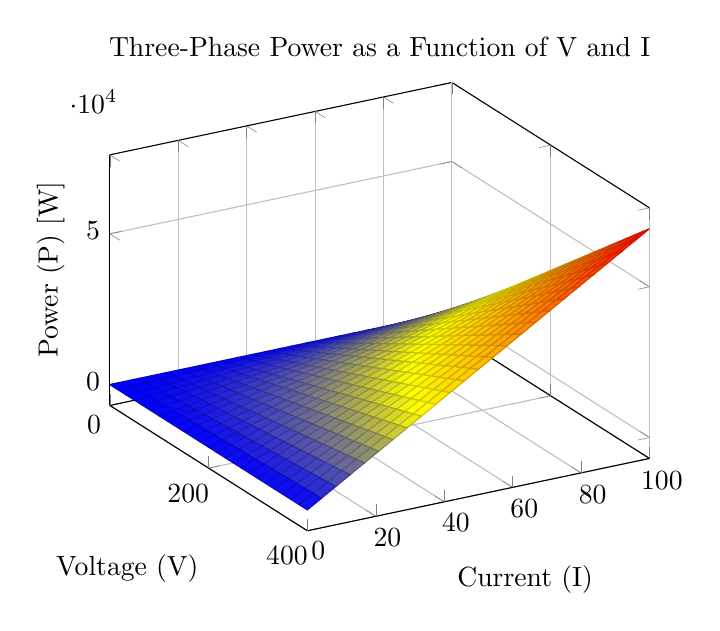
\begin{tikzpicture}
        \begin{axis}[
            title={Three-Phase Power as a Function of V and I},
            xlabel={Voltage (V)},
            ylabel={Current (I)},
            zlabel={Power (P) [W]},
            grid=major,
            view={60}{30}, % Adjusts the viewing angle
        ]
        \addplot3[
            surf,
            domain=0:400, % Range for Voltage (x-axis)
            domain y=0:100, % Range for Current (y-axis)
        ]
        {sqrt(3) * x * y};
        \end{axis}
    \end{tikzpicture}
    \caption{A 3D surface representing three-phase power based on voltage and current.}
    \label{fig:power_surface}
\end{figure}

% --- Diameter vs. Maximum Voltage Graph ---
\begin{figure}[htbp]
    \centering
    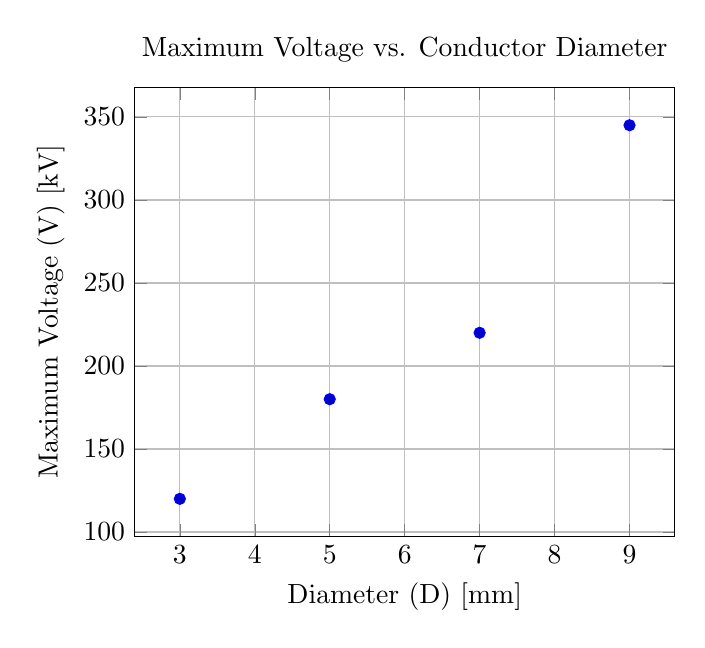
\begin{tikzpicture}
        \begin{axis}[
            title={Maximum Voltage vs. Conductor Diameter},
            xlabel={Diameter (D) [mm]},
            ylabel={Maximum Voltage (V) [kV]},
            grid=major,
            ]
        \addplot+[only marks] coordinates {
            (3, 120)
            (5, 180)
            (7, 220)
            (9, 345)
        };
        \end{axis}
    \end{tikzpicture}
    \caption{Relationship between conductor diameter and the maximum rated voltage it can support.}
    \label{fig:diameter_voltage}
\end{figure}

% --- Conductor Strength Bar Chart ---
\begin{figure}[htbp]
    \centering
    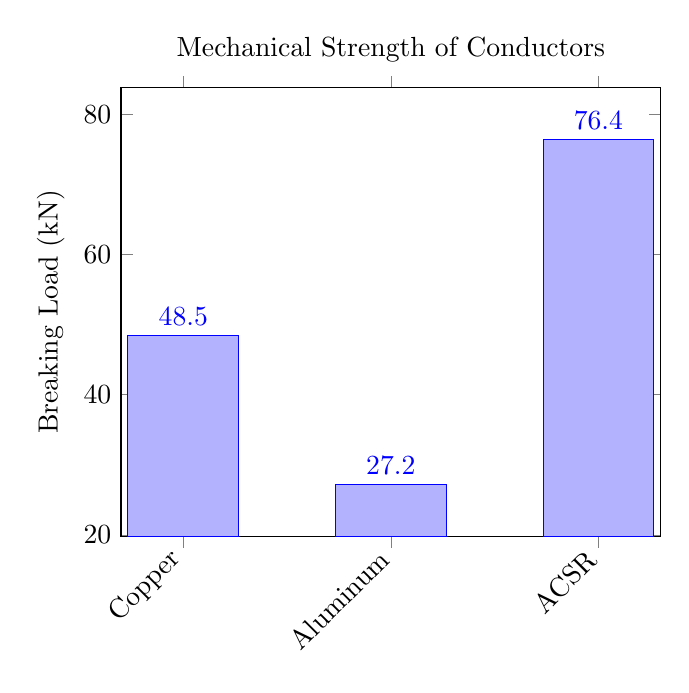
\begin{tikzpicture}
        \begin{axis}[
            title={Mechanical Strength of Conductors},
            ybar, % This creates a bar chart
             bar width=40pt,
            enlargelimits=0.15,
            ylabel={Breaking Load (kN)},
            symbolic x coords={Copper, Aluminum, ACSR},
            xtick=data,
            nodes near coords, % Shows the value on top of the bar
            nodes near coords align={vertical},
            x tick label style={rotate=45, anchor=east},
        ]
        \addplot coordinates {
            (Copper, 48.5)
            (Aluminum, 27.2)
            (ACSR, 76.4)
        };
        \end{axis}
    \end{tikzpicture}
    \caption{A comparison of the calculated breaking load for different conductor materials of similar cross-section.}
    \label{fig:strength_chart}
\end{figure}

\end{document}